\chapter{پیاده‌سازی و ارزیابی روش پیشنهادی}
\newpage
\ExplSyntaxOn
\cs_set_eq:NN
\etex_iffontchar:D
\tex_iffontchar:D
\cs_undefine:N \c_one
\int_const:Nn \c_one { 1 }
\ExplSyntaxOff
\setdigitfont{XB Zar}
\section{مقدمه}
در این فصل به ارزیابی روش پیشنهادی بر روی مجموعه‌ی مدارهای کوانتومی مختلف پرداخته شده است. در ابتدا کتابخانه‌های مورد استفاده معرفی شده و سپس روش‌های موجود که روش پیشنهادی با آن‌ها مقایسه شده است، معرفی می‌گردند. همچنین جهت ارزیابی روش پیشنهادی با سایر روش‌ها، چندین معیار معرفی خواهند شد. در انتها نتایج بدست آمده از روش پیشنهادی با سایر روش‌ها به همراه تجزیه و تحلیل نتایج و بیان نقاط قوت و ضعف هر روش ارائه می‌گردد\cite{andreev2006balanced}.

الگوریتم‌های پیشنهادی روی یک کامپیوتر کلاسیک با 8 گیکابایت حافظه‌ی رم و پردازنده‌ای 5 هسته‌ای بر روی نرم افزار متلب اجرا گردیدند.
\section{مجموعه مدارهای مورد استفاده}
همانطور که در فصل‌های پیشین بیان گردید، به دلیل محدودیت در پیاده سازی دروازه‌های چندکیوبیتی، نیاز است تا در مدارهای کوانتومی، دروازه‌های بیشتر از دو کیوبیت توسط دروازه‌های تک کیوبیتی و دو کیوبیتی جایگزین شوند. مجموعه کتابخانه‌ی مورد استفاده در این رساله، مجموعه‌ی دروازه‌های پایه  شامل دروازه‌های \lr{CNOT} و تک کیوبیتی‌ها می‌باشد.
% روش سنتز مورد استفاده جهت تبدیل دروازه‌های مدار به مجموعه دروازه‌های کتابخانه‌ای روش برگرفته از \cite{Barenco95} می‌باشد. شکل‌‎های \ref{figa5} و \ref{figb5} مدارهای جایگزین دروازه‌های سه و چهارکیوبیتی را نشان می‌دهند.



% \begin{figure}[h]
%\centering     
%\subfigure[مدار جایگزین دروازه‌های سه کیوبیتی در الگوریتم پیشنهادی ]{\label{figa5}\includegraphics[width=80mm]{2qubit.jpg}}
%\subfigure[مدار جایگزین دروازه‌های چهار کیوبیتی در الگوریتم پیشنهادی]{\label{figb5}\includegraphics[width=90mm]{3qubit.jpg}}
%\label{circuitre}
%\end{figure}




مجموعه مدارهای مورد استفاده جهت ارزیابی روش پیشنهادی در شش مجموعه دسته بندی شد و ویژگی‌های آن‎ها در جدول \ref{charachter} ارائه شده است.
\begin{table}[h]
\centering
\caption{وِیژگی مدارهای مورد استفاده}
\label{charachter}
\begin{tabular}{c|c|c|c|c}

نام &شماره‌ی مدارها& کتابخانه& تعداد کیوبیت‌ها& تعداد دروازه‌ها\\
\hline
مجموعه مدار 1 &9-1&\cite{maslov2005reversible} &$[480,1650]$&$[15,6430]$\\
\hline
مجموعه مدار 2 &15-10&\cite{Wille} &$[5,107]$&$[15,6430]$\\
\hline
مجموعه مدار 3&25-16&\cite{cross2017open}&$[10,40]$&$[40,500]$\\
\hline
مجموعه مدار 4&31-26&\cite{Wille}&$[4,17]$&$[7,110]$\\
\hline
مجموعه مدار 5&37-32&\cite{Wille} &$[480,1650]$&$[7,110]$\\
\hline
مجموعه مدار 6& 39-37&\cite{fowler2004scalability}, \cite{childs2003quantum}, \cite{whitfield2011simulation} &$[10,1000]$&$[10,1000]$\\

\end{tabular}
\end{table}




همچنين روش پیشنهادی با روش‌های ارائه شده در زیر مقایسه خواهد شد:
\begin{itemize}
\item
روش مبتنی بر پنجره ارائه شده توسط \cite{nikahd2021automated}: در این روش مدلی مبتنی بر روش برنامه‌ريزي خطی جهت افرازبندی گراف در نظر گرفته شده است وبه بهینه‌سازی سطح دوم نپرداخته است.
\item
روش افرازبندی مبتنی بر ابر گراف ارائه شده در \cite{Pablo}: در این روش مدار کوانتومی به ابرگراف تبدیل شده و ابرگراف افرازبندی می‌شود. دراین روش بهینه‌سازی سطح دوم بررسی نشده و تنها دروازه‌های متوالی که در کیوبیت کنترلی با یکدیگر اشتراک داشته‌اند، مورد نظر قرار گرفته است.
\item
روش افرازبندی مبتنی بر الگوریتم ژنتیک \cite{ZomorodiE}: در این روش افرازبندی مدار کوانتومی در دو زیر سیستم انجام شده و برای چند افراز مورد بررسی قرار نگرفته است.
\item
روش کاهش تعداد دورنوردی های کوانتومی ارائه شده در  \cite{Zomorodi}: در این مطالعه مسئله‌ی کاهش تعداد ارتباط‌های مورد نیاز جهت ارتباط در دو زیر سیستم مورد بررسی قرار گرفته و بهینه‌سازی سطح دوم جهت کاهش تعداد دورنوردی‌های مورد نیاز در دو افراز مورد بررسی قرار گرفته است.
\end{itemize}

\section{بررسی روش پیشنهادی بر روی مدار \lr{2-4dec}} 

در ابتدا الگوریتم پیشنهادی روی مدار  \lr{2-4dec} که از مجموعه‌ي مدارهای موجود در کتابخانه‌ی\lr{revlib} گرفته شده، اعمال خواهد شد. این مدار شامل 27 دروازه و 6 کیوبیت می‌باشد. الگوریتم پیشنهادی کیوبیت‌های مدار را در سه زیر سیستم توزیع خواهد نمود. شکل \ref{dec2-4} مدار کوانتومی مورد نظر را نشان می‌دهد. 
 
شکل \ref{dec2-41} مدار حاصل از افرازبندی سطح اول را نشان می‌دهد. در این افرازبندی، مجموعه کیوبیت‌های $\{q_6,q_4\}$ در افراز اول، $\{q_3,q_5 \}$ در افراز دوم و $\{q_6,q_4 \}$ در افراز سوم قرار گرفته‌اند. در افرازبندی حاصل، دروازه‌های سراسری شامل مجموعه‌ دروازه‌های $\{g_7,g_8,g_9,g_{10},g_{11},g_{12},g_{13},g_{14},g_{17},g_{18},g_{21},g_{24},g_{25}\}$ می‌باشد. همانطور که در فصل پیشین بیان گردید، تعداد کل ارتباط‌ها مورد نیاز دوبرابر تعداد دروازه‌های سراسری می‌باشد. در این مدار تعداد کل ارتباط‌ها ايجاد شده برابر 26 خواهد بود. پس از آن آرایه $P$ بدست آمده از این مرحله با مقدار [3,3,2,1,2,1]، به‌عنوان ورودی مرحله‌ي بعد داده می‌شود.
جدول \ref{tableexam} مراحل اجرای سطح دوم الگوریتم پیشنهادی را نشان می‌دهد. در این جدول، ستون 1 بیانگر شماره‌ی مرحله، ستون دو بیانگر اندیس $s$، نوع دروازه‌ی $g_s$  (تک کیوبیتی/ محلی/ سراسری) و کیوبیتی که دورنورد می‌شود، می‌باشد. همچنین در ستون سه افرازی که کیوبیت قرار است به آن دورنورد شود (افراز مقصد)، اندیس $d$ و افرازی که کیوبیت مجدد به آن باز می‌گردد (افراز مبدا) گزارش شده است. در ستون‌های چهارم و پنجم مقادبر آرایه‌های $run$ و $P$ در هر مرحله بیان شده است. این مراحل به صورت زیر می‌باشد:
 \begin{figure}
\centering     
\subfigure[مدار \lr{2-4dec}]{\label{dec2-4}\includegraphics[width=100mm]{4dec1}}
\subfigure[مدار حاصل از افرازبندي]{\label{dec2-41}\includegraphics[width=100mm]{4dec2}}
\caption{مثالی از افرازبندی مدار کوانتومی}
\label{Dec}
\end{figure}

\begin{itemize}
\item
مرحله‌ی اول: در این مرحله دروازه‌های $g_1 $ تا $g_6 $ دروازه‌های تک کیوبیتي بوده و اجرا می‌شوند و نیاز به هیچ دورنوردی کوانتومی نمی‌باشد. بنابراین $run[i]=1, i \in \{1,2,...,6\} $ مقداردهی می‌شود.
\item
مرحله‌ی دوم: دروازه‌ی $g_7(q_1,q_4)$ دروازه‌ای سراسری می‌باشد. کیوبیت $q_1 $ از افراز $P_3 $ به افراز $P_1 $ دورنورد می‌شود. با  دورنورد شدن این کیوبیت دروازه‌ی $g_{10}$ اولین دروازه‌ی سراسری است که در کیوبیت $q_1 $ با دروازه‌ی $g_{7}$ مشترک می‌باشد. اما از آنجایی‌که دروازه‌ی $g_{10}$ به دروازه‌ $g_{9}$ وابسته بوده و  $run[9]=0$ می‌باشد، بنابراین دروازه‌ی $g_{10}$ نمی‌تواند اجرا شود. و تنها دروازه‌ی $g_7$ اجرا شده و  $run[7]=1$ قرار می‌گیرد. درنهایت کیوبیت $q_1 $ به افراز $P_3 $ باز می‌گردد.

\item
مرحله‌ی سوم: دروازه‌ی $g_8(q_3,q_4)$ دروازه‌ای سراسری می‌باشد. کیوبیت $q_3 $ از افراز $P_2 $ به افراز $P_1 $ دورنورد می‌شود. با دورنورد شدن این کیوبیت، دروازه‌ی $g_{9}$ اولین دروازه‌ی سراسری است که در کیوبیت $q_3 $ با دروازه‌ی $g_{8}$ مشترک می‌باشد. بنابراین $run[i]=1,i \in\{8,9\}$ مقداردهی می‌شود و کیوبیت $q_3 $ به افراز خود بر می‌گردد.
\item
مرحله‌ی چهارم: دروازه‌ی $g_{10}(q_1,q_4)$ دروازه‌ای سراسری می‌باشد. کیوبیت $q_1 $ از افراز $P_3 $ به افراز $P_1 $ دورنورد می‌شود. هیچ دروازه‌ای دارای کیوبیت مشترک با دروازه‌ی $g_{10}$ نمی‌باشد. بنابراین $run[10]=1$ مقداردهی شده و در نهایت  $q_1$ به افراز  $P_3$ برمی‌گردد.
\item
مرحله‌‌ی پنجم: دروازه‌ی  $g_{11}(q_1,q_3)$ دروازه‌ی سراسری می‌باشد. کیوبیت $q_1 $ از افراز $P_3 $ به افراز $P_2 $ دورنورد می‌شود. هیچ دروازه‌ای دارای کیوبیت مشترک با دروازه‌ی $g_{11}$ نمی‌باشد. بنابراین $run[11]=1$ مقداردهی شده و در نهایت  $q_1$ به افراز  $P_3$ برمی‌گردد.
\item
مرحله‌ی ششم: دروازه‌ی  $g_{12}(q_3,q_4)$ دروازه‌ی سراسری می‌باشد. کیوبیت $q_4 $ از افراز $P_1 $ به افراز $P_2 $ دورنورد می‌شود. دروازه‌ی $g_{13}$ اولین دروازه‌ی سراسری بوده که در کیوبیت  $q_4 $ با دروازه‌ی $g_{12}$ مشترک است. این دروازه‌ بدون وابستگی به دروازه‌ای دیگر می‌تواند اجرا شود. بنابراین $run[i]=1,i \in \{12,13\}$ مقداردهی شده و  کیوبیت  $q_4$ به افراز مبدا خود باز می‌گردد.
\item
مرحله‌ی هفتم: دروازه‌ی  $g_{14}(q_2,q_3)$ دروازه‌ی سراسری می‌باشد. کیوبیت $q_2 $ از افراز $P_3 $ به افراز $P_2 $ دورنورد می‌شود. دروازه‌‌های $g_{18}$ و $g_{17}$ دروازه‌هایی هستند که در کیوبیت $q_2$ با دروازه‌ی $g_{14}$ مشترک بوده. از آنجایی که این دو دروازه محلی بوده، اجرا شده و در نتیجه دروازه‌ی $g_{18}$ نیز می‌تواند اجرا گردد. بنابراین $run[i]=1, i \in \{14,...,18\}$ مقداردهی شده و در نهایت کیوبیت  $q_2$ به افراز $P_3$ باز می‌گردد.
\item
مراحل هشتم و نهم: دروازه‌های $g_{19}$ و $g_{20}$ دروازه‌های محلی بوده و بدون نیاز به دورنوردی کوانتومی این دو دروازه اجرا می‌شوند. در نتیجه $run[i]=1,i \in \{19,20\}$ مقداردهی می‌شوند.

\item
مرحله‌ی دهم: دروازه‌ی  $g_{21}(q_2,q_4)$ دروازه‌ی سراسری بوده و کیوبیت $q_2$ به افراز $P_1$ دورنورد می‌شود. با این دورنوردی، دروازه‌های $g_{24} $ و $g_{25}$ می توانند اجرا شوند. بنابراین $run[i]=1,i \in \{21,...,25\}$ مقداردهی شده و در نهایت کیوبیت $q_2 $ به مبدا خود باز می‌گردد.
\item
مراحل یازدهم و دوازدهم: دروازه‌های $g_{26}$ و $g_{27}$ دروازه‎های محلی بوده و بدون نیاز به دورنوردی کوانتومی اجرا می‌شوند. بنابراین  $run[i]=1,i \in \{26,27\}$ مقداردهی می‌شوند.

\end{itemize} 
در مثال ذکر شده، هر یک از مراحل 1، 2، 3، 4، 5، 6 و 9 نیاز به دو دورنوردی کوانتومی دارند. بنابراین تعداد دورنوردی‌ها برابر 14 می‌باشد. بنابراین با اعمال بهینه سازی سطح دوم بر افرازبندی سطح اول تعداد دورنوردی‌های حدودا به نصف کاهش یافت.

\begin{table}
\begin{center}
\caption{مراحل اجرای الگوریتم روی مدار \lr{2-4dec}}
\label{tableexam}
\footnotesize{
\begin{tabular}{|c|c|c|c|c|}
\hline
مراحل&$g_s$&مقصد&$run$&$P$\\
\cline{2-2}\cline{3-3}
&حالت&$g_d$&&\\
\cline{2-3}
&$q\_teleport$&مبدا&&\\
\hline
0&&-&$[0,0,0,0,0,0,0,0,0,0,0,0,0,0,0,0,0,0,0,0,0,0,0,0,0,0,0]$&$[3,3,2,1,2,1,1]$\\[10pt]

\hline
&$g_1$&-&&\\
\cline{2-3}
1&تک کیوبیتی&$-$&$[\textcolor[rgb]{0.00,0.50,1.00}{1,1,1,1,1,1},0,0,0,0,0,0,0,0,0,0,0,0,0,0,0,0,0,0,0,0,0]$&$[3,3,2,1,2,1,1]$\\
\cline{2-3}
&$-$& $-$&&\\
\hline

&$g_7$&$P_1$&&\\
\cline{2-3}
2&سراسری&$g_{10}$&$[1,1,1,1,1,1,\textcolor[rgb]{0.00,0.50,1.00}{1},0,0,0,0,0,0,0,0,0,0,0,0,0,0,0,0,0,0,0,0]$&$[\textcolor[rgb]{0.00,0.50,1.00}{1},3,2,1,2,1,1]$\\
\cline{2-3}
&$q_1$& $P_3$&&\\
\hline
&$g_8$& $P_1$&&\\
\cline{2-3}
3&سراسری&$g_9$&$[1,1,1,1,1,1,1,\textcolor[rgb]{0.00,0.50,1.00}{1,1},0,0,0,0,0,0,0,0,0,0,0,0,0,0,0,0,0,0]$&$[3,3,\textcolor[rgb]{0.00,0.50,1.00}{1},1,2,1,1]$\\
\cline{2-3}
&$q_3$&$P_2$&&\\
\hline
&$g_{10}$&$P_1$&&\\
\cline{2-3}
4&سراسری&$g_{10}$&$[1,1,1,1,1,1,1,1,1,\textcolor[rgb]{0.00,0.50,1.00}{1},0,0,0,0,0,0,0,0,0,0,0,0,0,0,0,0,0]$&$[\textcolor[rgb]{0.00,0.50,1.00}{1},3,2,1,2,1,1]$\\
\cline{2-3}
& $q_1$& $P_3$&&\\
\hline
&$g_{11}$& $P_2$&&\\
\cline{2-3}
5&سراسری&$g_{11}$&$[1,1,1,1,1,1,1,1,1,1,\textcolor[rgb]{0.00,0.50,1.00}{1},0,0,0,0,0,0,0,0,0,0,0,0,0,0,0,0]$&$[\textcolor[rgb]{0.00,0.50,1.00}{2},3,2,1,2,1,1]$\\
\cline{2-3}
&$q_1$&$P_3$&&\\
\hline
&$g_{12}$&$P_2$&&\\
\cline{2-3}
6&سراسری&$g_{13}$&$[1,1,1,1,1,1,1,1,1,1,1,\textcolor[rgb]{0.00,0.50,1.00}{1,1},0,0,0,0,0,0,0,0,0,0,0,0,0,0]$&$[3,3,2,\textcolor[rgb]{0.00,0.50,1.00}{2},2,1,1]$\\
\cline{2-3}
& $q_4$&$P_1$&&\\
\hline
&$g_{14}$&$P_2$&&\\
\cline{2-3}
7&سراسری&$g_{18}$&$[1,1,1,1,1,1,1,1,1,1,1,1,1,\textcolor[rgb]{0.00,0.50,1.00}{1,1,1,1,1},0,0,0,0,0,0,0,0,0]$&$[3,\textcolor[rgb]{0.00,0.50,1.00}{2},2,1,2,1,1]$\\
\cline{2-3}
& $q_2$&$P_3$&&\\

\hline
&$g_{19}$& -&&\\
\cline{2-3}
8&محلی&-&$[1,1,1,1,1,1,1,1,1,1,1,1,1,1,1,1,1,1,\textcolor[rgb]{0.00,0.50,1.00}{1},0,0,0,0,0,0,0,0]$&$[3,3,2,1,2,1,1]$\\
\cline{2-3}
&-& -&&\\
\hline
&$g_{20}$& -&&\\
\cline{2-3}
9&محلی&-&$[1,1,1,1,1,1,1,1,1,1,1,1,1,1,1,1,1,1,1,\textcolor[rgb]{0.00,0.50,1.00}{1},0,0,0,0,0,0,0]$&$[3,3,2,1,2,1,1]$\\
\cline{2-3}
&-& -&&\\
\hline
&$g_{21}$& $P_1$&&\\
\cline{2-3}
10&سراسری&$g_{25}$&$[1,1,1,1,1,1,1,1,1,1,1,1,1,1,1,1,1,1,1,1,\textcolor[rgb]{0.00,0.50,1.00}{1,1,1,1,1},0,0]$&$[3,\textcolor[rgb]{0.00,0.50,1.00}{1},2,1,2,1,1]$\\
\cline{2-3}
&$q_{2}$& $P_3$&&\\
\hline
&$g_{26}$& $-$&&\\
\cline{2-3}
11&محلی&-&$[1,1,1,1,1,1,1,1,1,1,1,1,1,1,1,1,1,1,1,1,1,1,1,1,1,\textcolor[rgb]{0.00,0.50,1.00}{1},0]$&$[3,3,2,1,2,1,1]$\\
\cline{2-3}
&-& -&&\\
\hline

&$g_{27}$& -&&\\
\cline{2-3}
12&محلی&-&$[1,1,1,1,1,1,1,1,1,1,1,1,1,1,1,1,1,1,1,1,1,1,1,1,1,1,\textcolor[rgb]{0.00,0.50,1.00}{1}]$&$[3,3,2,1,2,1,1]$\\
\cline{2-3}
&-& -&&\\
\hline
\end{tabular}
}
\end{center}
\end{table}


\section{معیارهای ارزیابی روش پیشنهادی}
در این بخش به معرفی معیارها و پارامترهایی برای ارزیابی روش پیشنهادی پرداخته شده است. برای ارزیابی روش پیشنهادی با الگوریتم‌های موجود معیارهای زیر مورد استفاده قرار گرفته است. 
\begin{itemize}
\item
در معیار $R_1 $، نسبت تعداد دورنوردی‌های کوانتومی به تعداد دروازه‌های دو کیوبیتی مدار، مورد ارزیابی قرار می‌گیرد. از آنجایی که هر کیوبیتی که از مبدا خود دورنورد می‌شود، بایستی به مقصد خود باز گردد، در مخرج آن تعداد دروازه‌ها دو برابر شده است. این معیار در بازه‌ي $[0,1]$ بوده و به صورت معادله‌ی \eqref{R1} تعریف می‌شود.
\begin{equation}
R_1=\frac{N_t}{2*N_g}
\label{R1}
\end{equation}

در بدترین افرازبندی مدار کوانتومی، هر دروازه‌ی دو کیوبیتی در مدار، ممکن است به‌صورت یک دروازه‌ی سراسری در نظر گرفته شود و به تعداد دو برابر دروازه‌های دو کیوبیتی در مدار، ارتباط نیاز باشد. در نتیجه نسبت تعداد دورنوردی‌های بدست آمده از روش پیشنهادی به دو برابر تعداد دروازه‌های دو کیوبیتی، می‌تواند نشان دهنده‌ی عملکرد روش پیشنهادی باشد. هرچه این معیار به صفر نزدیکتر باشد، بیانگر این است که کاهش تعداد دورنوردی‌ها بهتر بوده و الگوریتم بهتر عمل نموده است.
\item
جهت نشان دادن تاثیر بهینه‌سازی سطح دوم بر افرازبندی سطح اول، معیار $R_2 $ به صورت معادله‌ی \eqref{R2} تعریف شده است.
\begin{equation}
R_2=\frac{N_t}{2*N_{non}}*100
\label{R2}
\end{equation}
این معیار بیان می‌کند بهینه‌سازی سطح دوم چه انداره تاثیر بر افرازبندی سطح اول داشته است. بنابراین درصد نسبت تعداد دورنوردی‌های بدست آمده از سطح دوم به دو برابر تعداد دروازه‌های سراسري بدست آمده از سطح اول، می‌تواند جهت نشان دادن میزان بهبودی که بهینه‌سازی سطح دوم بر سطح اول داشته است، استفاده شود. هر چه این میزان به صفر نزدیک‌تر باشد، نشان دهنده‌ی بهبود بیشتر است.

\item
جهت نشان دادن متوسط تعداد دورنوردی‌های مورد نیاز به ازای هر کیوبیت، معیار $R_3 $ به صورت معادله‌ی \ref{R4} تعریف شده است.
\begin{equation}
R_3=\frac{N_t}{N_q}
\label{R4}
\end{equation}
در این معادله، نسبت فضای مورد نیاز برای دورنوردی‌های کوانتومی به تعداد کیوبیت‌های موجود در سیستم نشان داده شده است. این معیار بیان می‌کند که به طور متوسط به ازای هر کیوبیت چه تعداد دورنوردی کوانتومی مورد نیاز است. هر چه میزان $R_3 $ از یک بیشتر باشد، بیانگر این است که به طور متوسط به ازای هر کیوبیت نیاز به یک دورنوردی کوانتومی می‌باشد. هر چه این میزان از یک کمتر باشد، به این معناست که کیوبیت‌های بیشتری با یکدیگر به طور محلی در تعامل بوده و توزیع کیوبیت‌ها به طور متوسط خوب عمل کرده است. هرچه این میزان از یک بیشتر باشند، به معنای توزیع نامناسب کیوبیت‌ها در افرازها بوده و به این معناست به طور متوسط برخی کیوبیت‌ها بیشتر از یکبار دورنوردی می‌شوند.
\item

 جهت ارزیابی و مقایسه با سایر روش‌ها، معیار انحراف استاندارد \footnote{\lr{Standard Deviation Criterion}} به صورت معادله‌ی \ref{Dev}  تعریف شده است:
\begin{equation}
Dev=\frac{T_{ap}-T_{best}}{T_{best}}*100
\label{Dev}
\end{equation}

\end{itemize}



در این معادله  $T_{best}$ بهترین تعداد دورنوردی‌های کوانتومی بدست آمده در میان روش‌ها روی مدار مورد نظر و $T_{ap}$ بیانگر تعداد دورنوردی‌های کوانتومی روشی است که می‌خواهیم مقایسه نماییم. چنانچه در بین روش‌هایی که در حال مقایسه هستیم، روشی دارای مقدار $Dev$ برابر صفر باشد، آنگاه دارای عملکرد بهتری در بین سایر روش‌ها است. هر چه میزان $Dev$ بیشتر بوده، نشان دهنده‌ی ضعیف عمل نمودن روش می‌باشد.


\section{آزمایش اول}

\begin{table}
\begin{center}
\caption{تعداد دورنوردی‌های کوانتومی حاصل از الگوریتم پیشنهادی در مقایسه با روش \cite{nikahd2021automated}}
\label{ta2}
\begin{tabular}{ccccccccccc}
\hline
شماره‌ي مدار&نام مدار&$N_{q}$ & $N_g$&$K$& روش پیشنهادی && روش ارائه شده در \cite{nikahd2021automated}&\\
&&&&&$N_t$&\lr{Dev}&$N_t$&\lr{Dev}\\
\cline{6-9}
1&$$\lr{2of5-D1}&6&104&2&40&0&40&0\\
2&\lr{2-4dec}&6&21&3 &14&27&11&0\\
3&\lr{6sym} &10&72&2&14&0&16&14\\
4&\lr{9sym}&12&108&3&22&0&36&63\\
5&\lr{8bitadder}&24&338&6&46&0&84&82\\
6&\lr{Cycle17\_3}&20&5861&3&2262&11&2028&0\\
7&\lr{Ham15-D3}&15&220 &4&144&29&101&0\\
8&\lr{Hwb50}&56&6430&4&1272&0&1301&2\\
9&\lr{Hwb100}&107&6430&4&2014&0&2513&24\\
10&\lr{Rd32 272}&5&5&2&4&0&6&50\\
11&\lr{Ham7\_106}&7&49&4&34&13&30&0\\
12&\lr{Rd53\_139}&8&49&2&8&0&12&50\\
13&\lr{Rd53\_311}&13&104&3&16&0&22&37\\
14&\lr{Parity 247}&17&16&3&6&50&4&0\\
15&\lr{Adder16\_174}&49 &200&3&6&0&9&50\\
\hline
\end{tabular}
\end{center}
\end{table}
در این آزمایش، الگوریتم پیشنهادی برروی مجموعه مدارهای 1 و 2 با شماره‌ي 1 تا 15 اعمال شد و با روش مبتنی بر پنجره ارائه شده در  \cite{nikahd2021automated} مقایسه گردید. جدول \ref{ta2} تعداد دورنوردی‌های کوانتومی بدست آمده از روش پیشنهادی در مقایسه با روش \cite{nikahd2021automated} بر روی اين مجموعه نشان می‌دهد.


\begin{table}
\centering
\caption{مقادیر $R_1$، $R_2$ و $R_3$  برای مجموعه داده‌های  1}
\label{tabler3}
\begin{tabular}{cccccc}
\hline
شماره‌ي مدار &نام مدار&$R_1$&$R_2$&$R_3$\\
\hline
1&\lr{2of5-D1}&$0.2$&40&$3.3$\\
2&\lr{2-4dec}&$0.33$&53&$1.1$\\
3&\lr{6sym} &$0.1$&22&$0.7$\\
4&\lr{9sym}&$0.18$&19&$0.92$\\
5&\lr{8bitadder}&$0.06$&21&$0.96$\\
6&\lr{Cycle17\_3}&$0.19$&30&$56.55$\\
7&\lr{Ham15-D3}&$0.35$&62&$5.13$\\
8&\lr{Hwb50}&$0.06$&23&$8.03$\\
9&\lr{Hwb100}&$0.15$&32&$9.42$\\
10&\lr{Rd32 272}&$0.4$&20&$0.4$\\
11&\lr{Ham7\_106}&$0.35$&53&$2.4$\\
12&\lr{Rd53\_139}&$0.1$&10&$0.5$\\
13&\lr{Rd53\_311}&$0.8$&20&$0.62$\\
14&\lr{Parity 247}&$0.1$&30&$0.17$\\
15&\lr{Adder16\_174}&$0.015$&43&$0.6$\\
\hline
\end{tabular}
\end{table}
در این جدول، ستون‌های 2 تا 6 به‌ترتیب نام مدار، تعداد کیوبیت‌ها، تعداد کل دروازه‌ها، تعداد دروازه‌های دو کیوبیتی و تعداد افرازهای موجود را بیان می‌نماید. همچنین در دیگر ستون‌ها مقدار $N_t$ و $ِDev$ برای الگوریتم پیشنهادی و روش مبتنی بر پنجره ارائه شده توسط \cite{nikahd2021automated} گزارش شده است. با توجه به رابطه‌ی \ref{Dev}، مقدار صفر برای این معیار بیانگر بهتر عمل نمودن روش نسبت به سایر روش‌هاست. همانطور که این جدول نشان می‌دهد، بجز در پنج مدار از مجموع 15 مدار، کارایی روش پیشنهادی نسبت به روش بیان شده در \cite{nikahd2021automated} بهتر بوده است.

جدول \ref{tabler3} مقادیر $R_1 $، $R_2 $ و $R_3 $ بدست آمده از روش پیشنهادی روی مدارهای 1 تا 15 نشان می‌دهد. از آنجایی‌که روش پیشنهادی\cite{nikahd2021automated} یک روش تک سطحی بوده و مرحله‌ی افرازبندی مدار از بهینه‌سازی تعداد دورنوردی‌ها جدا نبوده است، برای کار آن‌ها مقادیر $R_2 $ و $R_3 $ وجود ندارد.  همان‌طور که این جدول نشان می‌دهد، مدار \lr{8bitadder} دارای کمترین مقدار $R_1 $ در این 15 مدار بوده است که به معنای آن است که روش پیشنهادی به‌طور کارا این مدار را افراز نموده و منجر به کمترین تعداد دورنوردی کوانتومی شده است. همچنین مدار \lr{Cycle17\_3} دارای بیشترین مقدار $R_3 $ در بین سایر مدارات داشته است. که نشان دهنده‌ی آن بوده است که به طور متوسط هر کیوبیت 56 بار دورنورد شده است و بیانگر این است که ساختار مدار طوری بوده است که دروازه‌های دو کیوبیتی  مدار بیشترین وابستگی را به لحاظ محدودیت‌های پیش‌نیازی به یکدیگر داشته‌اند.

همچنین جهت نشان دادن میزان تاثیر بهینه‌سازی سطح دوم بر افرازبندی سطح اول، در هر مجموعه، نموداری ارائه شده است که درصد تعداد دورنوردی‌های مورد نیاز به تعداد دورنوردی‌های غیر نیاز را نشان مي‌دهد. نمودار\ref{figure7} تعداد دورنوردی‌های مورد نیاز به دورنوردی‌های غیر نیاز را برای مجموعه مدارهای 1 تا 15 نشان می‌دهد.
\begin{figure}
\centering
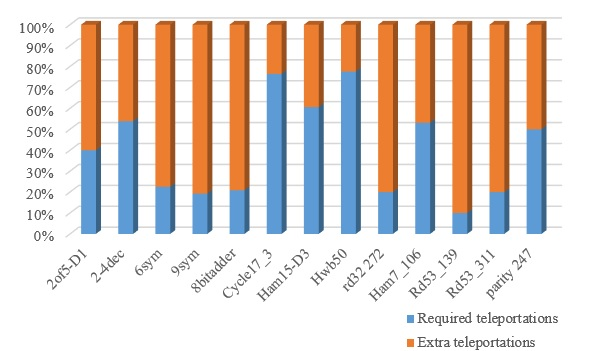
\includegraphics[scale=0.7]{figure7.jpg}
\caption{درصد دورنوردي‌هاي مورد نياز به دورنوردي‌هاي غير نياز}
\label{figure7}
\end{figure}
قسمت پایین این نمودار (رنگ آبی) تعداد دورنوردی های مورد نیاز پس از اعمال بهینه سازی سطح دوم بر افرازبندی سطح اول الگوریتم پیشنهادی را نشان می‌دهد. قسمت بالای نمودار (رنگ نارنجی) تعداد دورنوردی‌های غیر نیاز که از سطح اول بدست آمده است، نشان می‌دهد. همان‌طور که در فصل پیشین بیان گردید، تعداد ارتباط‌ها حاصل از افرازبندی سطح اول برابر تعداد برش‌های موجود یا همان تعداد دروازه‌های سراسری می‌باشد. به میزان نمودار نارنجی رنگ این تعداد دروازه‌های سراسری با اعمال بهینه‌سازی سطح دوم می‌تواند به صورت محلی و بدون نیاز به دورنوردی کوانتومی اجرا گردد. بیش از 70 درصد دروازه‌های سراسری حاصل از سطح اول به صورت محلی اجرا می‌گردد.
یک توزیع ساده \footnote{\lr{naive}} به ازای هر دروازه‌ی سراسری نیاز به يك دورنوردی کوانتومی دارد. هر چه اختلاف بین تعداد دروازه‌های سراسری و تعداد دورنوردی‌های کوانتومی بیشتر باشد، نشان دهنده‌ی کاهش بیشتر تعداد دورنوردی‌های مورد نیاز به تعداد ارتباط‌های مورد نیاز از سطح اول است. 
%برای نمونه در شکل مدار \lr{GSE} برای افراز \lr{K=13} توزیع متعادل نداشته است.


\section{آزمایش دوم}

در آزمایش دوم روش پیشنهادی روی مجموعه مدارهای شماره 3 تست شد و با الگوریتم پیشنهادی توسط \cite{nikahd2021automated} مقایسه گردید. تعداد دورنوردی‌های بدست آمده از دو روش در جدول \ref{table4} گزارش شد. در این جدول نام مدار، تعداد کیوبیت‌ها، تعداد کل دروازه‌ها، تعداد افرازها و معيار $Dev$ به‌ترتیب در ستون‌های دو تا شش گزارش شده است. همانطور که این جدول نشان می‌دهد، به جز در سه مدار با شماره‌های 17، 18 و 23 کارایی روش پیشنهادی نسبت به روش دیگر بهتر بوده است. همچنین ستون‌هایی که $N_t$ در آن گزارش شده است، نشان می‌دهد که با افزایش تعداد دروازه‌های مدار، تعداد دورنوردی‌های کوانتومی در دو روش افزایش یافته است.  
\begin{table}
\centering
\caption{مقایسه تعداد دورنوردی‌های بدست آمده از روش پیشنهادی با روش پیشنهادی در \cite{nikahd2021automated}.}
\label{table4}
\begin{tabular}{ccccccccc}
\hline

شماره‌ي مدار&نام مدار&$N_{q}$ &$N_g$&$K$& روش پیشنهادی & & روش  \cite{nikahd2021automated}&\\
&&&&&$N_t$&\lr{Dev}&$N_t$&\lr{Dev}\\
\cline{6-9}
\hline
16&[[10-3-3]]&10&44&2&\textbf{12}&0&13&8\\
17&[[16-3-5]]&16&89&4&64&33&\textbf{48}&0\\
18&[[21-1-7]]&21&140&3&68&22&\textbf{56}&0\\
19&[[24-3-7]]&24&205&4&\textbf{86}&0&101&17\\
20&[[25-1-9]]&25&168&5&\textbf{72}&0&88&22\\
21&[[27-1-9]]&27&110&4&\textbf{96}&0&98&2\\
22&[[31-1-16]]&31&339&4&\textbf{126}&0&138&9\\
23&[[33-1-9]]&33&316&4&184&33&\textbf{138}&0\\
24&[[35-1-10]]&35&389&4&\textbf{116}&0&120&3\\
25&[[40-3-10]]&40&483&4&\textbf{162}&0&184&13\\
\hline
\end{tabular}
\end{table}
همچنین میزان تاثیر بهینه‌سازی سطح دوم بر افرازبندی سطح اول در شکل \ref{extra2} براي اين مجموعه نشان داده شده است. همان‌طور که این نمودار نشان می‌دهد، از میله‌های دو تا سه از سمت چپ و میله‌های شش تا ده با افزایش تعداد دروازه‌های دو کیوبیتی مدار، این نسبت با کاهش مواجه بوده است و نشان دهنده‌ی این است که روش پیشنهادی توانسته است عملکرد مناسبی بر روی کاهش معیار $R_2 $ داشته باشد.
\begin{table}
\centering
\label{table5}
\caption{معیارهای $R_1$ تا $R_3$ برای مجموعه داده‌های شماره‌ي 3 }
\begin{tabular}{cccccccc}
\hline
شماره‌ي مدار& نام مدار&$N_{2qubit}$&$N_{non}$ & $N_t$ & $R_1 $& $R_2 $& $R_3 $ \\
\hline
16&[[10-3-3]]&37&16&12&$0.16$&$37.5$&$0.6$\\
17&[[16-3-5]]&76&53&64&$0.42$&60&2\\
18&[[21-1-7]]&120&69&68&$0.28$&50&$1.6$\\
19&[[24-3-7]]&140&117&86&$0.31$&37&$1.8$\\
20&[[25-1-9]]&145&58&72&$0.25$&62&$1.44$\\
21&[[27-1-9]]&219&64&96&$0.22$&75&$1.78$\\
22&[[31-1-16]]&319&103&126&$0.2$&62&2\\
23&[[33-1-9]]&284&155&184&$0.33$&60&$2.79$\\
24&[[35-1-10]]&355&101&116&$0.16$&55&$1.66$\\
25&[[40-3-10]]&446&150&162&$0.18$&54&2\\
\hline
\end{tabular}
\end{table}
\begin{figure}
\centering
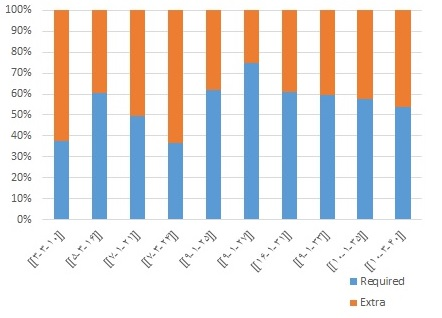
\includegraphics[scale=0.9]{extra2.jpg}
\caption{درصد دورنوردي‌هاي مورد نياز به دورنوري‌هاي غير نياز براي مجموعه  مدارهاي شماره 3}
\label{extra2}
\end{figure}


\section{آزمایش سوم}
در آزمایش دیگر، اثر تعداد افرازها بر روی تعداد دورنوردی‌های کوانتومی بر روي مجموعه مدارهای \lr{GSE} ، \lr{QFT} و \lr{BWT} مورد بررسی قرار گرفت. همچنین جهت ارزیابی و مقایسه روش پیشنهادی با روش ارائه شده در \cite{Pablo}، از معیار نسبت تعداد دورنوردی‌ها به تعداد کیوبیت‌ها که به صورت معادله‌ی \ref{R4} ارائه گردید، استفاده شده است.

 \begin{figure}
\centering     
\subfigure[مدار\lr{BWT} ]{\label{bwt}\includegraphics[width=80mm]{BWT.jpg}}
\subfigure[مدار\lr{QFT}]{\label{qft}\includegraphics[width=80mm]{qft.jpg}}
\subfigure[مدار\lr{GSE}]{\label{gse}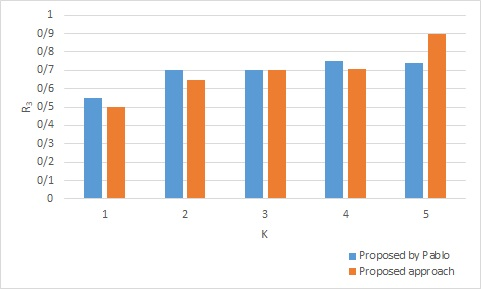
\includegraphics[width=80mm]{GSE.jpg}}

\caption{ارزیابی روش پیشنهادی با الگوریتم ارائه شده در \cite{Pablo} برای مدارهای \lr{BWT}، \lr{QFT} و \lr{GSE} برروی معیار $R_3$}
\label{figure71}
\end{figure}


در نمودار \ref{figure71}، هر میله بیانگر معیار $R_3 $ برای روش پیشنهادی و روش ارائه شده در \cite{Pablo} بوده و محورهای \lr{X} و \lr{Y} به‌ترتیب بیانگر تعداد افرازها و $R_3 $ برای مدارهای \lr{BWT}، \lr{QFT} و \lr{GSE} می‌باشند. در مقایسه با الگوریتم ارائه شده در \cite{Pablo}، روش آن‌ها دارای مراحل اضافی پیش پردازش و پس پردازش بوده و این دو مرحله برای الگوریتم آن‌ها سربار اضافی ایجاد نموده است. در این نمودار معیار $R_4 $ برای تمامی مدارها و افرازها بجز برای مدار \lr{GSE} در تعداد افراز \lr{K=13} نسبت به دیگر روش بهتر عمل نموده است. همچنین در مدار \lr{GSE}  در تعداد افراز \lr{{K=7}} به طور مشابه با این روش عمل کرده است. این مقادیر در جدول \ref{table6} نیز نشان داده شده است. همانطور که این جدول نشان می‌دهد، مدار \lr{QFT} در روش \cite{Pablo} دارای توزیع مناسبی نبوده است. زیرا در این مدار به ازای ${K>5}$ مقدار \lr{R} بیشتر از یک شده است و این بیانگر این است که به طور متوسط هر کیوبیت بیشتر از یک بار دورنوردي شده است. 

\begin{table}
\begin{center}
\caption{ معیار $R_3$ حاصل از روش پیشنهادی در مقایسه با روش ارائه شده در \cite{Pablo} }
\label{table6}
\footnotesize{
\begin{tabular}{cp{0.4cm}p{0.4cm}p{0.01cm}p{0.4cm}p{0.4cm}p{0.01cm}p{0.4cm}p{0.4cm}p{0.01cm}p{0.3cm}p{0.3cm}p{0.01cm}p{0.3cm}p{0.3cm}p{0.01cm}p{0.3cm}p{0.3cm}}
&\lr{K=3}&&&\lr{K=5}&&&\lr{K=7}&&&\lr{K=9}&&&\lr{K=11}&&&\lr{K=13}&\\
\cline{2-3} \cline{5-6}\cline{8-9} \cline{11-12}\cline{14-15}\cline{17-18}
نام مدار&$R_4$&$R_4$\cite{Pablo}&&$R_4$& $R_4$\cite{Pablo}&&$R_4$& $R_4$\cite{Pablo}&&$R_4$&$R_4$\cite{Pablo}&&$R_4$&$R_4$\cite{Pablo}&&$R_4$&$R_4$\cite{Pablo}\\
\hline
\lr{BWT}&$0.12$&$0.55$&&$0.35$&$0.6$&&$0.35$&$0.64$&&$0.7$&$0.65$&&$0.35$&$0.7$&&$0.36$&$0.77$\\
\lr{QFT}&$0.4$&1&&$0.85$&$1.4$&&$1.2$&$1.58$&&$1.2$&$1.75$&&$1.6$&$1.75$&&$1.75$&$1.8$\\
\lr{GSE}&$0.5$&$0.54$&&$0.64$&$0.7$&&$0.7$&$0.7$&&$0.79$&$0.8$&&$0.72$&$0.74$&&$0.9$&$0.74$\\
\end{tabular}
}

\end{center}
\end{table}

نمودار شکل \ref{figure8} نسبت تعداد دورنوردی‌های کوانتومی به تعداد دروازه‌های سراسری در مقایسه با روش \cite{Pablo} بر روی مدار \lr{QFT} زمانی‌که مدار روی تعداد افرازهای$ K\in\{2,4,6,...,16\}$ توزیع شود، نشان می‌دهد. هرچه این نسبت از یک کمتر باشد، بیانگر این است که اعمال بهینه‌سازی سطح دوم تاثیر بیشتری در افرازبندی سطح اول داشته است و کیوبیت‌ها بهتر توزیع شده‌اند.
\begin{figure}
\centering
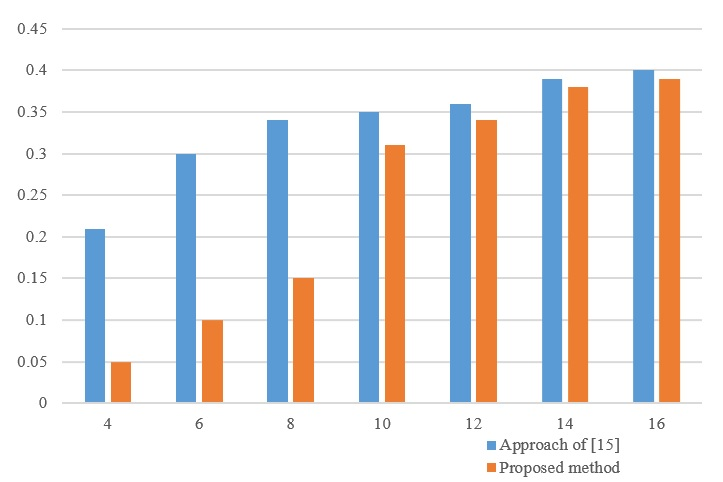
\includegraphics[scale=0.6]{figure8.jpg}
\caption{سهم تعداد دورنوردی‌های مورد نیاز در مقایسه با تعداد دروازه‌های سراسری برروی مدار \lr{QFT} برای تعداد افرازهای $K \in\{2,4,...,16\}$}
\label{figure8}
\end{figure}


توزیع مدار در افرازهای بیشتر بیانگر تعداد دروازه‌های سراسری بیشتر و افزایش تعداد دورنوردی‌های کوانتومی است. از این نمودار دو نکته قابل درک است:
\begin{itemize}
\item
با افزایش تعداد افرازها تعداد دورنوردی‌های کوانتومی در هر دو روش روبه افزایش می‌باشد. 
\item
در تمامی موارد الگوریتم پیشنهادی نسبت به روش ارائه شده در \cite{Pablo} بهتر عمل کرده است، که این نشان دهنده‌ی این است که الگوریتم پیشنهادی تعداد بیشتری از دروازه‌های سراسری را به صورت محلی اجرا نموده است.
\end{itemize}
\section{آزمایش چهارم}
در آزمایشی دیگر اثر فاکتور توازن بار $\omega$ بر روی تعداد ارتباط‌ها بین زیر سیستم‌های کوانتومی مورد بررسی قرار گرفت. همانطور که در فصل پیشین بیان گردید، جهت آن‌که کیوبیت‌ها بین سیستم‌ها به طور متوازن توزیع گردند، در مدل برنامه‌ریزی خطی ارائه شده، نامعادله‌ی \ref{load} در افرازبندی اضافه گردید:
\begin{equation}
|V_{i}|\leq \frac{(1+\omega )|V|}{K}\\
\forall i \in \{1,...,K\}
\label{load}
\end{equation}
در این نامعادله، هر چه این فاکتور به صفر نزدیکتر باشد، کیوبیت‌ها دارای توازن بیشتری در زیر سیستم‌ها بوده و به طور متوازن بین آن‌ها توزیع شده‌اند. اما هرچه این فاکتور بزرگتر باشد، کیوبیت‌ها نامتوازن‌تر بین سیستم‌ها توزیع می‌شوند. در این آزمایش اثر این فاکتور روی توزیع کیوبیت‌ها نشان داده شده است. شکل \ref{omega} میزان تاثیر فاکتور $\omega$ بر روی تعداد دروازه‌های سراسری بدست آمده از افرازبندی سطح اول را نشان می‌دهد. این آزمایش برای مقادیر متفاوت $\omega \in \{0.1,...,0.9\} $ مورد بررسی قرار گرفت.
\begin{figure}
\centering
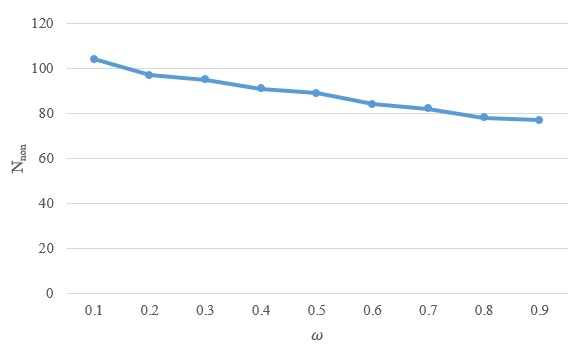
\includegraphics[scale=0.6]{omega.jpg}
\caption{ تاثیر ضریب توازن بار بر روی تعداد ارتباط‌ها بین زیر سیستم‌ها} 
\label{omega}
\end{figure}
همان‌طور که این نمودار نشان می‌دهد، با افزایش مقدار $\omega$ تعداد دروازه‌های سراسری یا همان تعداد ارتباط‌ها سطح اول کاهش می‌یابد. زیرا با افزایش مقدار $\omega$ کیوبیت‌ها نامتوازن‌تر بین سیستم‌ها توزیع شده و در نتیجه کیوبیت‌هایی که بیشتر با یکدیگر در ارتباط هستند، در یک افراز قرار گرفته و  دروازه‌ی بین آن‌ها به صورت محلی اجرا می‌گردد که نتیجه آن کاهش تعداد ارتباط‌ها بین زیر سیستم‌هاست. بیشترین تعداد دروازه‌های سراسری برای مقدار $\omega=0.1 $ بدست آمده است.
\section{آزمایش پنجم}
جهت مقایسه با روش‌های ارائه شده در \cite{Zomorodi} و \cite{ZomorodiE}، الگوریتم پیشنهادی روی مجموعه مدارهای شماره‌ی 5 آزمایش شد. نتایج بدست آمده در جدول  \ref{table8} نشان داده شده است. ستون‌ 6 از این جدول بیانگر تعداد دروازه‌های سراسری از افرازبندی سطح اول الگوریتم پیشنهادی بوده است. در ستون‌های 7 و 8 مقدار $N_t$ برای روش‌های \cite{Zomorodi} و \cite{ZomorodiE} نشان داده شده است. همان طور که این جدول نشان می‌دهد، در تمام مدارهای این مجموعه، الگوریتم پیشنهادی دارای عملکرد بهتری بوده است.

\begin{table}
\begin{center}
\caption{نتایج بدست آمده از الگوریتم پیشنهادی در مقایسه با روش های ارائه شده در \cite{ZomorodiE}، و\cite{Zomorodi} }
\label{table8}
\footnotesize{
\begin{tabular}{cccccp{0.5cm}p{0.5cm}p{0.5cm}p{0.5cm}}
\hline
شماره مدار&نام مدار&$N_{q}$&$N_g$&$K$&$N_t$  \cite{davarzani}&$N_t$  \cite{Zomorodi}&$N_t$ \cite{ZomorodiE}&$N_t$ \\
\hline
26&\lr{Pariaty\_247}&17 &16&2&2&2&2&2\\
27&\lr{Sym9\_147}&12&108&2&8&\lr{N.A.}&48&6\\
28&\lr{Flip\_flop}&8&30&3&8&\lr{N.A.}&\lr{N.A.}&8\\
29&\lr{Alu\_primitive}&6 &21&2&6&18&20&2\\
30&\lr{Alu\_primitive\_opt}&6 &21& 2 &6& 10& 10& 4\\
31&\lr{Figure 4 of \cite{Zomorodi}}&4&7 &2 &2 &4 &4 &2\\
\hline
\end{tabular}
}
\end{center}
\end{table}

\section{آزمایش ششم}
همچنین مدل پیشنهادی روی مجموعه مدارهای بزرگتر اجرا گردید. تعداد کیوبیت‌های این مدارها در بازه‌ی $[500,1600] $ و تعداد دروازه‌های مدار در بازه‌ی $[500,1600] $ بود جهت ارزیابی و بررسی سیستم مورد نظر برای این مجموعه مدارها، تعداد افرازها نیز در بازه‌ی $[3,50] $ در نظر گرفته شد. جدول \ref{table7} تعداد دورنوردی‌های کوانتومی بدست آمده از الگوریتم پیشنهادی را برای این مجموعه مدارها و تعداد افراز متفاوت نشان می‌دهد.
\begin{table}
\begin{center}
\renewcommand{\arraystretch}{1.3}
\caption{\label{table7} نتایج بدست آمده از روش پیشنهادی روی مجموعه مدارهاي شماره‌ي 6 و تعداد افرازهای متفاوت}
\footnotesize{
\begin{tabular}{cccccccccccc}
\hline
شماره‌مدار&نام مدار&$N_{q}$ &$N_g$&هزینه مدار&&&&$K$&&&\\
\hline
&&&&&3&4&5&6&10&20&50\\
\cline{6-12}
32&\lr{Spla}&489&1709&5925&287&496&576&832&1925&2746&3418\\
33&\lr{Average of 16}&576&3484&7452&96&131&180&245&  1534&2283&4350\\
%Pdc&619&2080&6500&548&1146&1283&1532&3276&4078&4564\\
34&\lr{CPS}&923&2763&8487&548&1146&1283&1532&3276&4078&4564\\
35&\lr{Apex5}&1025&2909&10349&352&526&1158&1503&4980&5689&6321\\
36&\lr{Frg2}&1219&3724&12468&397&690&4419&4812&6088&6542&7162\\
37&\lr{Seq}&1617&5990&19362&457&2535&3458&6371&7716&20&50\\
\hline
\end{tabular}
}
\end{center}
\end{table}
شکل \ref{figure10} تاثیر تعداد افرازها روی تعداد دورنوردی‌های کوانتومی را برای سه مدار \lr{CPS}، \lr{ Apex5} و \lr{Frg2} نشان می‌دهد. با افزایش تعداد افرازها، مقدار $N_t$ افزایش یافته است. زیرا کیوبیت‌ها در تعداد افرازهای بیشتری توزیع شده و در نتیجه دروازه‌های بیشتری به صورت سراسری اجرا می‌گردند.

\begin{figure}
\centering
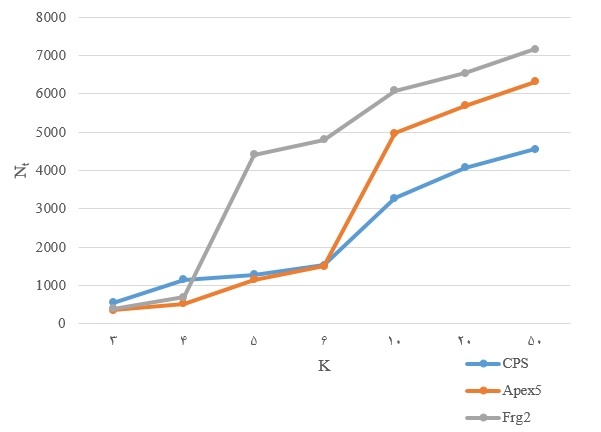
\includegraphics[scale=0.6]{huge.jpg}
\caption{تاثیر تعداد افرازها بر تعداد دورنوردی‌های کوانتومی روی سه مدار \lr{CPS}، \lr{ Apex5} و \lr{Frg2} }
\label{figure10}
\end{figure}
همچنین نمودارهای \ref{fig11} تاثیر اعمال بهینه‌سازی سطح دوم در افرازبندی سطح اول را برای مدارهاي بزرگ نشان می‌دهد. بیش از 60 درصد دروازه‌ها با اعمال سطح دوم به صورت محلی اجرا شده‌ و در نتیجه تعداد دورنوردی‌های کوانتومی کاهش یافته است.
 \begin{figure}
\centering     
\subfigure[]{\label{}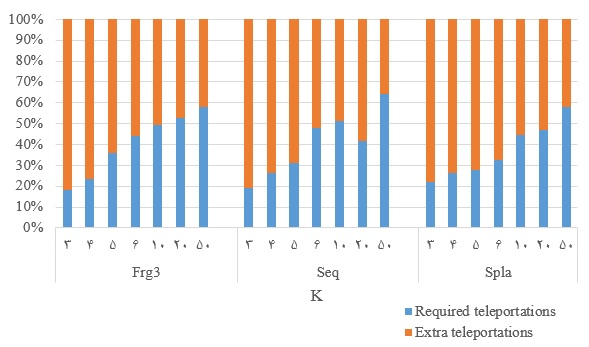
\includegraphics[width=80mm]{huge1.jpg}}
\subfigure[]{\label{}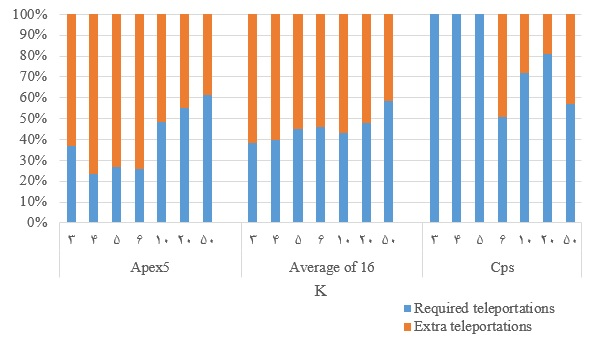
\includegraphics[width=80mm]{huge2.jpg}}
 \caption{تاثیر بهینه‌سازی سطح دوم بر افرازبندی سطح اول. نمودار آبی درصد دورنوردی‌های مورد نیاز و نمودار نارنجی درصد دورنوردی‌های اضافی را برای سه مدار \lr{CPS}، \lr{ Apex5} و \lr{Frg2} نشان می‌دهد.}
  \label{fig11}
  \end{figure}
\section{آزمایش هفتم}
در آزمایش آخر تاثیر دو روش ابتکاری ارائه شده، روی افرازبندی کیوبیت‌ها با استفاده از الگوریتم \lr{NSGA-III} که جهت افرازبندی آن‌ها در دو سیستم کوانتومی ارائه شد، نشان داده شده است. جدول \ref{table8} نتایج الگوریتم پیشنهادی را روی شش نمونه مدار نشان می‌دهد. در این جدول نتایج با الگوریتم‌های \lr{Random search} و الگوریتم ارائه شده در \cite{ZomorodiE} مقایسه شده است.
\begin{table}
\begin{center}
\renewcommand{\arraystretch}{1.3}
\caption{\label{table8} نتایج بدست آمده از روش پیشنهادی روی مجموعه مدارهاي 6 و تعداد افرازهای متفاوت}
\footnotesize{
\begin{tabular}{ccccccc}

نام مدار&$N_q$&$N_g$&$N_t(RS)$&$N_t$ &$N_t(I)$&$N_t(II)$\\
\hline
\lr{4gt5\_76}&5&11&18&14&4&8\\
\lr{Sym9\_147}&12&54&94&48&8&16\\
\lr{Parity\_47}&17&9&12&2&2&2\\
\lr{4Modulo7}&5&11&16&10&10&10\\
\lr{Figure 4 of \cite{Zomorodi}}&4&7&4&4&4&4\\
\lr{4-qubit QFT}&4&8&12&8&6&6\\
\end{tabular}
}
\end{center}
\end{table}

\section{خلاصه}
در این فصل، الگوریتم‌های پیشنهادی روی مجموعه‌ی مدارهاي مختلف آزمایش شد. برای مقایسه با سایر روش‌ها، چندین معیار ارزیابی معرفی و با چندین روش مقایسه گردید. در طی چندین آزمایش، عوامل متعدد مورد بررسی قرار گرفت. اولین بررسی‌های انجام شده، تاثیر افرازبندی سطح اول روی بهینه‌سازی سطح دوم که منجر به کاهش تعداد دروازه‌های سراسری گردید، بود. به عبارتی با انجام بهینه‌سازی سطح دوم تعدادی از دروازه‌های سراسری به طور محلی اجرا شدند که این امر تاثیر چشم‌گیری در کاهش تعداد دورنوردی‌های کوانتومی داشت. همچنین از بررسی‌های دیگری که انجام شد، بررسی تعداد دورنوردی‌های ایجاد شده به فضای کیوبیت‌های سیستم بود که هر چه این نسبت به یک نزدیکتر باشد، نشان دهنده‌ی این است که به طور متوسط هر کیوبیت یک بار دورنورد شده و هر چه این نسبت از یک بیشتر باشد نشان دهنده‌ی این است که به طور متوسط هر کیوبیت بیشتر از یکبار دورنورد شده است. همچنین اثر ضریب فاکتور توزیع بار روی کاهش تعداد دروازه‌های سراسری نشان داده شد. هر چه این فاکتور به صفر نزدیکتر باشد، توزیع متوازن کیوبیت‌ها در مدارها با افزایش تعداد دورنوردی‌های کوانتومی همراه است. در انتها الگوریتم پیشنهادی روی مجموعه مدارهاي بزرگتر که شامل تعداد کیوبیت‌ها و دروازه‌های بیشتر بود، آزمایش گردید. در مقایسه با سایر روش‌های بیان شده، الگوریتم‌های پیشنهادی دارای بهبود زیادی در کاهش تعداد دورنوردی‌های کوانتومی داشته‌ است.
